\documentclass[../report.tex]{subfiles}

\begin{document}

\graphicspath{{img/}{../img/}}

\section{Scrum men... Ikke helt}
\label{sec:Scrum}

Target-projektgruppen har valgt at arbejde med Scrum i deres implementeringsfase, hvilket optager cirka halvdelen af deres tidsplan(se Gantt diagram fig \ref{fig:Gantt} side \pageref{fig:Gantt}). I detes Scrum-forl�b blev det besluttet at k�re l�st p� nogle af Scrums discipliner, fordi der var enighed om at det ikke gav meget mening for en projektgruppe der kun m�des et par gange om ugen. En forklaring af target-projektgruppens Scrum aktiviteter ses p� tabel \ref{tab:Scrum} og de vigtige aktiviteters placering i sprintet p� figur \ref{fig:ScrumTimeline}.


\begin{figure}[H]
\centering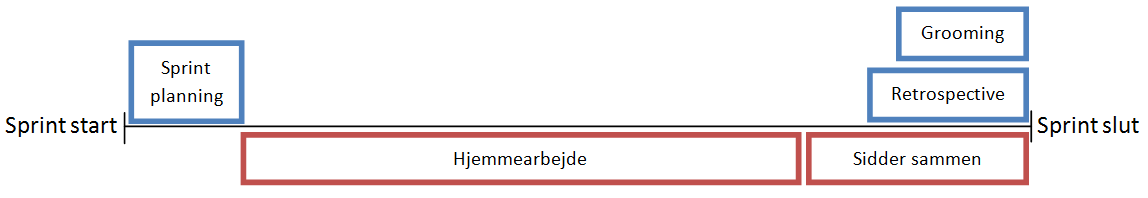
\includegraphics[scale=0.45]{SCRUMtimeLine.png}
\caption{Sprint tidslinje}
\label{fig:ScrumTimeline}
\end{figure}



%\noindent Target-projektgruppens sprints startede s�ledes med sprint planning, efterfulgt af en periode med individuelt arbejde, for s� at afslutte med gruppearbejde hvor Scrumboardet blev groomet og et retrospective p� sprintet udf�rt.


\begin{table}[H]
\begin{tabularx}{15cm}{l|X}
\textbf{Aktivitet}  & \textbf{Beskrivelse} \\
Scrum roller & I et eksamensprojekt er det urealistisk at have en person til kun at v�re product owner. I target-projektet er product owner ene og alene ansvarlig for kommunikation med stakeholders og prioritering af product items, men han er ogs� udvikler i Scrum teamet. Derudover er Scrummaster og developers blevet brugt klassisk.     \\ 
 & \\
Sprint & Sprints af 1 uges varighed\\
 & \\
Standup meeting & Der blev ikke afholdt nogen standup meetings. \\
 & \\
Grooming & Den n�stsidste aktivitet var grooming, hvor Scrumboardet blev ryddet op. \\
 & \\
Retrospective & Den sidste aktivitet var retrospective. Gruppen benyttede Keep-Stop-New metoden.\cite{cohn} \\
 & \\
Sprint planning & Den f�rste aktivitet i hvert sprint er en klassisk sprint planning. Tasks blev estimeret med planning poker i points som beskrevet i afsnit \ref{sec:Delphi} p� side \pageref{sec:Delphi}. \\
 & \\
Scrumboard & Scrum boardet er den centrale oversigt over aktiviteter. Da target-projektgruppen ikke havde et fast lokale allokeret, var et fysisk Scrumboard ikke muligt, s� online v�rkt�jet Trello(se trello.com) blev brugt i stedet. \\
 & \\
Tidtagning & Der blev i fire sprints taget tid p� arbejdet med Toggl(se toggl.com). Target-projektgruppen blev bedt om dette for hj�lp med analyse i dette projekt.
\end{tabularx}
\caption{Target-projektets Scrum aktiviteter}
\label{tab:Scrum}
\end{table}

\newpage

\noindent Target-projektgruppen har ikke brugt Scrum i hele deres projektforl�b, men det kunne de godt have valgt at g�re. De udtaler f�lgende:

\begin{quote}
\textit{"Grunden til at vi ikke har brugt Scrum fra projektstart er, at vi f�lte en hvis struktur af dokumentationen var n�devendig. Vi har alts� set p� Scrum som en implementerings procesmodel. I vores Scrum forl�b har vi dog ogs� haft andet end implementeringstasks, og vi ser sagtens gevinster ved at bruge Scrum fra projektstart."}
\end{quote}

\noindent Da den procesmodel som target-projektgruppen har brugt, nu er blevet udforsket, forts�tter vi i n�ste afsnit med at kigge p� vandfaldsmodellen og hvordan den kunne v�re et alternativ.


\end{document}